\section{Séries numériques et familles sommables}

\begin{solution}
	\phantom{}
	\begin{enumerate}
		\item On a $b_{0}=a_{1}=5,b_{1}=a_{3}=13$ et pour $p\geqslant2$, $b_{p}=2b_{p-1}+3b_{p-2}$.
		
		On a donc l'équation caractéristique $x^{2}-2x-3=0$. Les deux solutions sont 3 et -1. Donc il existe $(\lambda,\mu)\in\R^{2}$, $b_{p}=\lambda 3^{p}+\mu(-1)^{p}$.

		On a alors $b_{0}=5=\lambda+\mu$ et $b_{1}=13=3\lambda-\mu$. On trouve alors 
		$$\boxed{\lambda=\frac{9}{2} \text{ et } \mu=\frac{1}{2}}$$

		\item On le montre par récurrence sur $p\in\N$.
		
		\item Si $3^{p}\leqslant n<3^{p+1}$, on a $a_{n}=b_{p}=\frac{9}{2}3^{p}+\frac{1}{2}(-1)^{p}$.
		Alors 
		$$\frac{3}{2}+\frac{1}{2}(-1)^{p}\frac{1}{3^{p+1}}<\frac{a_{n}}{n}\leqslant\frac{9}{2}+\frac{1}{2}(-1)^{p}\frac{1}{3^{p}}$$
		Soit $\sigma\colon\N\to\N$ strictement croissante telle que 
		$$\frac{a_{\sigma(n)}}{\sigma(n)}\xrightarrow[n\to+\infty]{}\lambda$$
		Soit $p_{n}\in\N$ tel que $3^{p_{n}}\leqslant\sigma(n)<3^{p_{n}+1}$. On a 
		$$p_{n}=\bigl\lfloor\log_{3}(\sigma(n))\bigr\rfloor\xrightarrow[n\to+\infty]{}+\infty$$
		En reportant, on a $\frac{3}{2}\leqslant\lambda\leqslant\frac{9}{2}$.

		Si $\sigma(n)=3^{n}$, on a 
		$$\frac{a_{3^{n}}}{3^{n}}=\frac{b_{n}}{3^{n}}=\frac{9}{2}+\frac{1}{2}\frac{(-1)^{n}}{3^{n}}\xrightarrow[n\to+\infty]{}\frac{9}{2}$$
		Si $\sigma(n)=3^{n+1}-1$, on a 
		$$\frac{a_{3^{n}}}{3^{n}}=\frac{b_{n}}{3^{n+1}-1}\xrightarrow[n\to+\infty]{}\frac{3}{2}$$

		Soit $\mu\in[1,3[$ et $\sigma(n)=\lfloor 3^{n}\mu\rfloor\underset{n\to+\infty}{\sim}3^{n}\mu$. Alors 
		$$\frac{a_{\sigma(n)}}{\sigma(n)}=\frac{b_{n}}{\lfloor3^{n}\mu\rfloor}\underset{n\to+\infty}{\sim}\frac{b_{n}}{3^{n}\mu}=\frac{9}{2\mu}+\frac{1}{2\mu}\frac{(-1)^{n}}{3^{n}}\xrightarrow[n\to+\infty]{}\frac{9}{2\mu}$$
		
		$$\boxed{\text{Donc tout réel compris dans } \Biggl[\frac{3}{2},\frac{9}{2}\Biggr] \text{ est valeur d'adhérence.}}$$
	\end{enumerate}
\end{solution}

\begin{solution}
	\phantom{}
	\begin{enumerate}
		\item \function{g}{[a,b]}{\R}{x}{f(x)-x}
		est continue, $g(a)\geqslant0$ et $g(b)\leqslant0$, donc le théorème des valeurs intermédiaires affirme qu'il existe $l\in[a,b]$ avec $g(l)=0$, d'où 
		$$\boxed{f(l)=l}$$

		\item On note $A=\{\lambda\bigm| \lambda\text{ est valeur d'adhérence}\}$.
		Le théorème de Bolzano-Weierstrass indique que $A$ est non vide. De plus, $A$ est borné car $A\subset[a,b]$. Soit $\lambda=\inf(A)$ et $\mu=\sup(A)$. 
		
		Si $\lambda=b$, on a $\mu=b$ et $A=\{b\}=\{\lambda\}=\{\mu\}$.

		Si $\lambda<b$, soit $\varepsilon>0$. Si $\lambda\notin A$, $\{k\in\N\bigm| x_{k}\in]\lambda,\lambda+\varepsilon[\}$ est infini. Par définition, $\lambda$ est valeur d'adhérence. Donc $\lambda\in A$, et de même $\mu\in A$.

		Soit $\nu\in]\lambda,\mu[$ avec $\lambda<\mu$. Si $\nu\notin A$, il existe $\varepsilon_{0}>0$ tel que $\{k\in\N\bigm|\vert x_{k}-\nu\vert<\varepsilon_{0}\}$ est fini. Donc il existe $N_{0}\in\N$ tel que pour tout $n\geqslant N_{0}$, $x_{n}\notin]\nu-\varepsilon_{0},\nu+\varepsilon_{0}[$. Comme $\lim\limits_{n\to+\infty}\vert x_{n+1}-x_{n}=0$, il existe $N_{1}\in\N$ tel que pour tout $n\geqslant N_{1}$, $\vert x_{n+1}-x_{n}\vert<2\varepsilon_{0}$. 
		Soit alors $n\geqslant\max(N_{0},N_{1})$. Si $x_{n}\leqslant\nu-\varepsilon_{0}$, alors $x_{n+1}\leqslant\nu-\varepsilon_{0}$. Si $x_{n}\geqslant\nu+\varepsilon_{0}$, alors $x_{n+1}\geqslant\nu+\varepsilon_{0}$. Ceci contredit que $\lambda$ et $\mu$ sont valeur d'adhérence. 
		
		Ainsi, $\nu\in A$ et 
		$$\boxed{[\lambda,\mu] \text{ est le segment des valeurs d'adhérence.}}$$

		\item Si $(x_{n})$ converge, alors $\lim\limits_{n\to+\infty}x_{n+1}-x_{n}=0$. Réciproquement, si $\lim\limits_{n\to+\infty}x_{n+1}-x_{n}=0$, d'après 2., on a $A=[\lambda,\mu]$. On suppose $\lambda<\nu$. Ainsi, $\frac{\lambda+\nu}{2}=\alpha$ est valeur d'adhérence. Donc il existe $\sigma\colon\N\to\N$ strictement croissante telle que $x_{\sigma(n)}\xrightarrow[n\to+\infty]{}\alpha$. Alors $\lim\limits_{n\to+\infty}x_{\sigma(n)+1}=f(\alpha)$ par continuité de $f$ et c'est aussi égale à $\lim\limits_{n\to+\infty}x_{\sigma(n)}=\alpha$ car $\lim\limits_{n\to+\infty}x_{n+1}-x_{n}=0$.
		Ainsi, $$\boxed{f(\alpha)=\alpha}$$

		Par ailleurs, il existe $n_{0}\in\N$ tel que $x_{n_{0}}\in[\lambda,\mu]$ et $f(x_{n_{0}})=x_{n_{0}}\in A$, alors pour tout $n\geqslant n_{0}$, on a $x_{n}=x_{n_{0}}$. Donc $(x_{n})_{n\in\N}$ converge et $\lambda=\mu$: $(x_{n})_{n\in\N}$ est bornée et a une unique valeur d'adhérence. 
		$$\boxed{\text{Donc }(x_{n})_{n\in\N}\text{ converge.}}$$
	\end{enumerate}
\end{solution}

\begin{solution}
	On a $u_{n}=e^{\i 2^{n}\theta}$ pour tout $n\in\N$.

	Si $(u_{n})_{n\in\N}$ converge vers $l$, alors $\lim\limits_{n\to+\infty}u_{n}=1$ car $l=l^{2}$ et $\vert l\vert=1$.

	Si $(u_{n})_{n\in\N}$ est périodique au-delà d'un certain rang, il existe $T\in\N^{*}$, il existe $N_{0}\in\N$ tel que pour tout $n\geqslant N_{0}$, $u_{n+T}=u_{n}$. En particulier, $u_{N_{0}+T}=u_{N_{0}}$. On veut alors $2^{N_{0}+T}\theta\equiv 2^{N_{0}}\theta[2\pi]$. D'où $2^{N_{0}+T}\theta=2\theta+2k\pi$ donc $2^{N_{0}}(2^{T}-1)\theta=2k\pi$. Donc $\frac{\theta}{2\pi}\in\Q$.

	Réciproquement, si $\frac{\theta}{2\pi}\in\Q$, son développement binaire est périodique à partir d'un certain rang, et donc $(u_{n})_{n\in\N}$ l'est aussi.

	Si $(u_{n})_{n\in\N}$ est stationnaire, il existe $N\in\N$ tel que pour tout $n\geqslant N$, $U_{N+1}=U_{N}=U_{N^{2}}$. Comme $\vert U_{N}\vert=1$, alors $2^{n}\theta\in 2\pi\N$ et $\frac{\theta}{2\pi}$ est dyadique. 

	Réciproquement, s'il existe $p\in\N$, $u_{0}\in\N$ tel que $\frac{\theta}{2\pi}=\frac{p}{2^{n_{0}}}$ (nombre dyadique). Alors pour tout $n\geqslant n_{0}$, $2^{n}\theta\in 2\pi\N$ et $u_{n}=u_{n_{0}}=1$.

	Pour la densité, on prend une suite $(a_{n})_{n\in\N}$ en écrivant successivement, pour tout $k\in\N^{*}$, tous les paquets de $k$ entiers sont dans $\{0,1\}^{k}$. Soit $x\in[0,1[$ tel que 
	$$x=\sum_{n=1}^{+\infty}\frac{a_{n}}{2^{n}}$$
	Soit $N\in\N$, il existe $p_{N}\in\N$, 
	$$2^{p_{N}}\theta=2\pi\underbrace{(\dots)}_{\in\N}+2\pi(\frac{a_{1}}{2}+\dots+\frac{a_{N}}{2^{N}}+\underbrace{\dots}_{\in[0,\frac{1}{2^{N}}[})$$
	On a alors 
	$$e^{\i2^{p_{N}}\theta}=e^{\i2\pi(\frac{a_{1}}{2}+\dots+\frac{a_{N}}{2^{N}}+\dots)}$$
	et 
	$$\Bigl\vert\frac{a_{1}}{2}+\dots+\frac{a_{N}}{2^{N}}-x\Bigr\vert\leqslant\frac{1}{2^{N}}$$
	D'où $\lim\limits_{N\to+\infty}u_{p_{N}}=e^{\i2\pi x}$ et $(u_{n})_{n\in\N}$ est dense dans $\U$.
\end{solution}

\begin{solution}
	Si $a=0$ et $b=0$, $u_{n}\xrightarrow[n\to+\infty]{}0$.

	Si $a=0$ et $b\neq0$ (ou inversement), $u_{n}\underset{n\to+\infty}{\sim}\Bigl(\frac{1}{2}\Bigr)^{n^{2}}\xrightarrow[n\to+\infty]{}0$.

	Si $a>0$ ou $b>0$, on a
	\begin{align*}
		u_{n}
		&=\exp\Bigl(n^{2}\ln\Bigl(\frac{e^{\frac{1}{n}\ln(a)}+e^{\frac{1}{n}\ln(b)}}{2}\Bigr)\Bigr)\\
		&=\exp\Bigl(n^{2}\ln\Bigl(1+\frac{1}{2n}\ln(ab)+\frac{1}{4n^2}(\ln(a)^{2}+\ln(b)^{2})\Bigr)+o\Bigl(\frac{1}{n^{2}}\Bigr)\Bigr)\\
		&=\exp\Bigl(\frac{n}{2}\ln(ab)+\frac{1}{4}(\ln(a)^{2}+\ln(b)^{2}+o(1))\Bigr)
	\end{align*}

	Si $ab>1$, on a 
	$$\boxed{\lim\limits_{n\to+\infty} u_{n}=+\infty}$$
	
	Si $ab<1$, on a 
	$$\boxed{\lim\limits_{n\to+\infty} u_{n}=0}$$

	Si $ab=1$, on a 
	$$\boxed{\lim\limits_{n\to+\infty} u_{n}=e^{\frac{1}{2}\ln(a)^{2}}}$$
\end{solution}

\begin{solution}
	\phantom{}
	\begin{enumerate}
		\item Soit $M=\sup\limits_{n\in\N}x_{n}>0$ (car $\sum_{n\in\N}x_{n}=+\infty$). 
		$$J=\Biggl\{k\in\N\bigm| x_{k}\geqslant\frac{M}{2}\Biggr\}$$
		est fini car $x_{n}\xrightarrow[n\to+\infty]{}0$ et est non vide. On définit 
		$$\varphi(0)=\min\Biggl\{k\in J\Bigm| x_{k}=\max\{x_{n}\bigm|n\in J\}\Biggr\}$$
		Pour tout $n\in J$, $x_{\varphi(0)}\geqslant x_{n}$. Si $n\notin J$, $x_{n}\leqslant\frac{M}{2}<x_{\varphi(0)}$. Ainsi, 
		$$\boxed{x_{\varphi(0)}=\max\{x_{n}\bigm| n\in\N\}}$$
		Puis on recommence avec 
		$$\Bigl\{x_{n}\bigm| n\in\N\setminus\{\varphi(0)\}\Bigr\}$$

		\item Pour $l=0$, pour tout $\varepsilon>0$, il existe $n\in\N$ tel que $x_{N}<\varepsilon$. On pose 
		$$\boxed{I=\{N\}}$$
		et on a bien 
		$$\Biggl\lvert\sum_{k\in I}x_{k}-l\Biggr\rvert\leqslant\varepsilon$$

		Si $l=+\infty$, soit $A>0$. Il existe $N\in\N$ tel que $\sum_{k=0}^{N}x_{k}>A$ (car $\sum_{n\in\N}x_{n}=+\infty$). Donc on peut prendre 
		$$\boxed{I=\{0,\dots,N\}}$$

		Si $l\in\R_{+}^{*}$. Soit $\varepsilon>0$, on peut supposer sans perte de généralité que $\varepsilon<l$. Il existe $N_{0}\in\N$ tel que pour tout $n\geqslant N_{0}$, on a $x_{n}<\varepsilon$ et $\sum_{n=N_{0}}^{+\infty}x_{n}=+\infty$. Donc il existe un plus petit entier $N_{1}$ tel que $\sum_{n=N_{0}}^{N_{1}}x_{n}\geqslant l-\varepsilon$. Comme $x_{N_{1}}<\varepsilon$, on a $\sum_{n=N_{0}}^{N_{1}}x_{n}\leqslant l+\varepsilon$. Donc 
		$$\boxed{I=\{N_{0},\dots,N_{1}\}}$$
	\end{enumerate}
\end{solution}

\begin{solution}
	On pose 
	$$S_{n}=\sum_{k=0}^{n}u_{k}^{2}$$
	Montrons que $S_{n}\xrightarrow[n\to+\infty]{}+\infty$. D'abord, il existe $n_{0}\in\N$ tel que $u_{n_{0}}>$ donc $\lim\limits_{n\to+\infty}S_{n}=l\in\overline{R}_{+}^{*}$. Si $l<+\infty$, on a $u_{n}\xrightarrow[n\to+\infty]{}\frac{1}{l}$ et donc $u_{n}^{2}\xrightarrow[n\to+\infty]{}\frac{1}{l^{2}}$ et la série diverge. Donc $l=+\infty$ et comme $u_{n}\underset{n\to+\infty}{\sim}\frac{1}{S_{n}}$, on a $u_{n}\xrightarrow[n\to+\infty]{}0$.

	On observe ensuite que $S_{n}-S_{n-1}=u_{n}^{2}=o(1)$ donc $S_{n-1}\underset{n\to+\infty}{\sim}S_{n}$. Ainsi, 
	$$\underbrace{u_{n}^{2}S_{n}^{2}}_{=~(S_{n}-S_{n-1})S_{n}^{2}}\xrightarrow[n\to+\infty]{}1$$
	et on a 
	$$\frac{S_{n}^{2}+S_{n}S_{n-1}+S_{n-1}^{2}}{S_{n}^{2}}=1+\frac{S_{n-1}}{S_{n}}+\frac{S_{n-1}^{2}}{S_{n}^{2}}\xrightarrow[n\to+\infty]{}3$$
	donc 
	$$\underbrace{(S_{n}-S_{n-1})(S_{n}^{2}+S_{n}S_{n-1}+S_{n-1}^{2})}_{=~S_{n}^{3}-S_{n-1}^{3}}\xrightarrow[n\to+\infty]{}3$$

	On applique le théorème de Césaro à la suite $S_{n}^{3}-S_{n-1}^{3}$:
	$$\frac{S_{n}^{3}-S_{0}^{3}}{n}\xrightarrow[n\to+\infty]{}3$$
	donc $S_{n}\underset{n\to+\infty}{\sim}\sqrt[3]{3n}$, et comme $u_{n}\underset{n\to+\infty}{\sim}\frac{1}{S_{n}}$, on a bien 
	$$\boxed{u_{n}\underset{n\to+\infty}{\sim}\frac{1}{\sqrt[3]{3n}}}$$

	Réciproquement, soit $u_{n}=\frac{1}{\sqrt[3]{3n}}$ avec $u_{0}=1$. On a 
	$$u_{n}^{2}=\frac{1}{(3n)^{\frac{2}{3}}}$$
	Par comparaison série-intégrale, on a 
	$$\sum_{k=0}^{n}u_{k}^{2}\underset{n\to+\infty}{\sim}\frac{1}{3^{\frac{2}{3}}}\times 3n^{\frac{1}{3}}=(3n)^{\frac{1}{3}}$$
	et donc 
	$$\boxed{u_{n}\times\sum_{k=0}^{n}u_{k}^{2}\underset{n\to+\infty}{\sim}\frac{\sqrt[3]{3n}}{\sqrt[3]{3n}}=1}$$
\end{solution}

\begin{remark}
	On rappelle que l'on a la comparaison série-intégrale, pour $\alpha<1$,
	$$\sum_{k=1}^{N}\frac{1}{k^{\alpha}}\underset{n\to+\infty}{\sim}\int_{1}^{N}\frac{dt}{t^{\alpha}}\underset{n\to+\infty}{\sim}\frac{1}{1-\alpha}N^{1-\alpha}$$
\end{remark}

\begin{solution}
	Tout d'abord, on montre que pour tout $x\in[0,1]$,
	$$0\leqslant\cosh(x)-1-\frac{x^{2}}{2}\leqslant x^{4}$$
	en posant \function{f}{[0,1]}{\R}{x}{\cosh(x)-1-\frac{x^{2}}{2}}
	de classe $\mathcal{C}^{\infty}$ sur $[0,1]$ et on a $f''(x)=\cosh(x)-1\geqslant0$ et $f'(0)=0$. Comme $f(0)=0$, on a pour tout $x\in[0,1],f(x)\geqslant0$.

	Avec l'inégalité de Taylor-Lagrange à l'ordre 4 sur $f$, on a
	$$0\leqslant\cosh(x)-1-\frac{x^{2}}{2}\leqslant\frac{x^{4}}{24}\times\underbrace{\sup\limits_{t\in[0,1]}\vert\cosh^{(4)}(t)\vert}_{\leqslant\cosh(1)}\leqslant x^{4}$$

	\begin{figure}
		\centering
		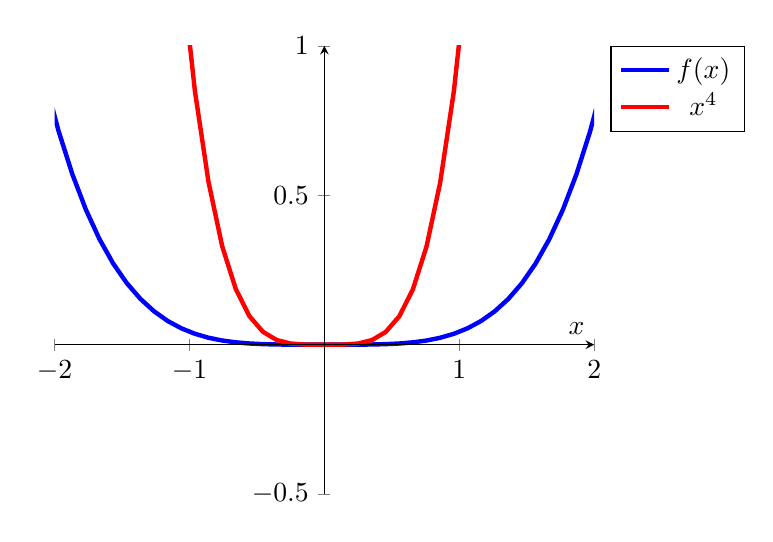
\begin{tikzpicture}
			\begin{axis}[
				xmin=-2, xmax=2,
				ymin=-0.5, ymax=1,
				axis lines=center,
				axis on top=true,
				xlabel=$x$,
				samples=100,
				legend pos=outer north east
			]
			\addplot[blue, ultra thick] {cosh(x)-1-x^2/2};
			\addplot[color=red, ultra thick, restrict y to domain=-1.5:1.5] {x^4};
			\legend{$f(x)$,$x^4$}
			\end{axis}
		\end{tikzpicture}
		\caption{$0\leqslant\cosh(x)-1-\frac{x^{2}}{2}\leqslant x^{4}$ pour $x\in\R$.}
	\end{figure}

	On a 
	$$-x_{n}=\sum_{k=1}^{n}\Bigl[\cosh\Bigl(\frac{1}{\sqrt{k+n}}\Bigr)-1\Bigr]$$
	Ainsi, 
	$$0\leqslant x_{n}-\sum_{k=1}^{n}\frac{1}{2}\frac{1}{n+k}\leqslant\sum_{k=1}^{n}\frac{1}{(n+k)^{2}}\leqslant\frac{n}{(n+1)^{2}}\xrightarrow[n\to+\infty]{}0$$

	On a 
	$$\sum_{k=1}^{n}\frac{1}{n+k}=H_{2n}-H_{n}=\ln(2n)+\gamma+o(1)-\ln(n)-\gamma=\ln(2)+o(1)$$
	Donc 
	$$\boxed{\lim\limits_{n\to+\infty}x_{n}=-\frac{\ln(2)}{2}}$$
\end{solution}

\begin{solution}
	$\varphi$ est dérivable sur $\R$ et on a pour tout $x\in\R$, $\varphi'(x)=e^{x}-1$.

	\begin{figure}[ht!]
		\centering
		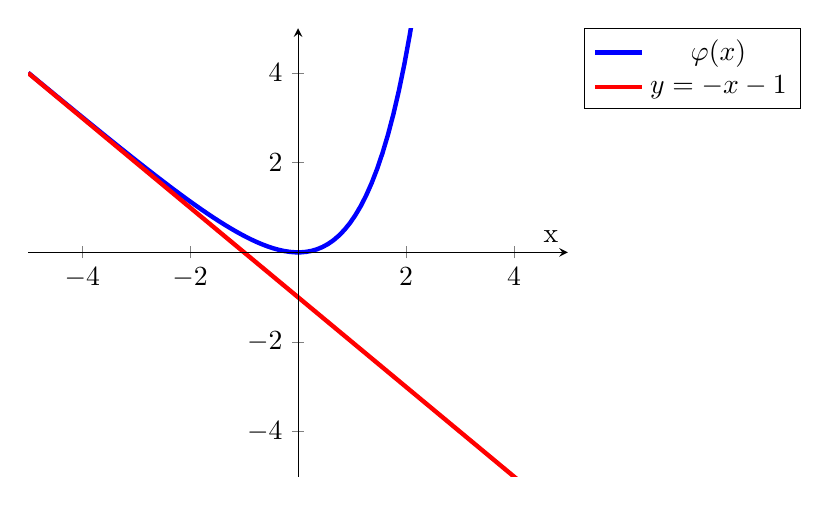
\begin{tikzpicture}
			\begin{axis}[
				xlabel=x,
				samples=100,
				xmin=-5, xmax=5, ymin=-5, ymax=5,
				legend pos=outer north east,
				axis lines=center,
				axis on top=true,]
				\addplot[blue, ultra thick] {e^x-x-1};
				\addplot[red, ultra thick] {-x-1};
				\legend{$\varphi(x)$,$y=-x-1$}
			\end{axis}
		\end{tikzpicture}
		\caption{$e^{x}-x-1\geqslant -x-1$ pour $x\in\R$.}
	\end{figure}

	On a 
	$$0\varphi(a_{n})\leqslant\varphi(a_{n})+\varphi(b_{n})+\varphi(c_{n})\xrightarrow[n\to+\infty]{}0$$
	donc $$\lim\limits_{n\to+\infty}\varphi(a_{n})=0$$

	Par l'absurde, soit $\varepsilon>0$. Supposons qu'il existe une infinité d'entiers $k\in\N$ tel que $\vert a_{k}\vert>\varepsilon$. Cela implique alors
	$$\varphi(a_{k})\geqslant\min(\varphi(\varepsilon),\varphi(-\varepsilon))>0$$
	ce qui contredit $\lim\limits_{n\to+\infty}\varphi(a_{n})=0$.
	Donc 
	$$\boxed{\lim\limits_{n\to+\infty}a_{n}=0}$$
	et c'est pareil pour $b_{n}$ et $c_{n}$.
\end{solution}

\begin{solution}
	\phantom{}
	\begin{enumerate}
		\item Soit \function{f}{]0,1[}{\R}{x}{x(1-x)}
		On a $f(x)\in]0,\frac{1}{4}]$. Pour tout $n\in\geqslant1$, $u_{n}\in]0,\frac{1}{4}]$. Par récurrence, on a donc $u_{n+1}\leqslant u_{n}$ et $\lim\limits_{n\to+\infty}u_{n}=0$. 
		
		$$\boxed{\text{Donc }v_{n}\text{ est bien définie.}}$$

		\begin{figure}[!ht]
			\centering
			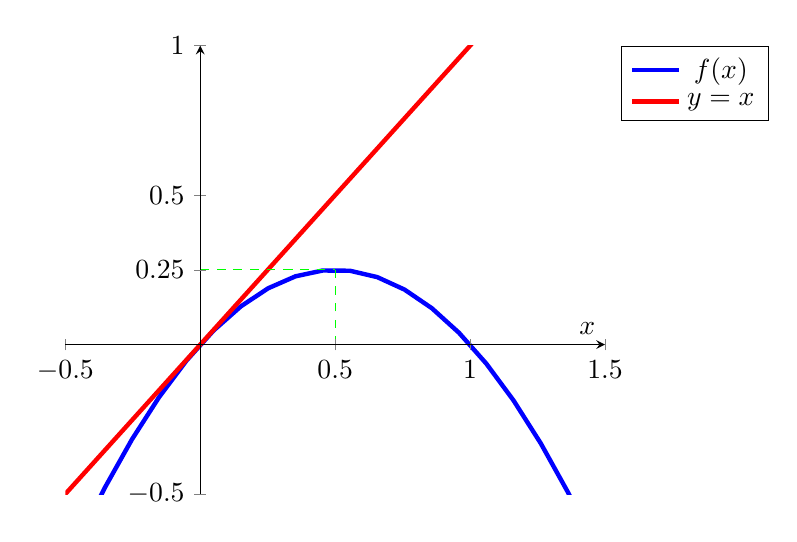
\begin{tikzpicture}
				\begin{axis}
					[
						xlabel=$x$,
						xmin=-0.5, xmax=1.5,
						ymin=-0.5, ymax=1,
						legend pos=outer north east,
						axis lines=center,
						axis on top=true,
						samples=100,
						extra y ticks={0.25}
					]
					\addplot[blue, ultra thick] {x*(1-x)};
					\addplot[red, ultra thick] {x};
					\addplot[green, dashed, domain=0:0.5] {0.25};
					\addplot[green, dashed, domain=0:0.5] coordinates {(0.5,0)(0.5,0.25)};
					\legend{$f(x)$,$y=x$}
				\end{axis}
			\end{tikzpicture}
			\caption{$x(1-x)\in\bigl]0,\frac{1}{4}\bigr]$ pour $x\in]0,1[$.}
		\end{figure}

		\item On a 
		$$\frac{1}{u_{n+1}}=\frac{1}{u_{n}}\times\frac{1}{1-u_{n}}=\frac{1}{u_{n}}(1+u_{n}+o(u_{n}))=\frac{1}{u_{n}}+1+o(1)$$
		Donc $v_{n+1}-v_{n}\xrightarrow[n\to+\infty]{}1$. D'après le théorème de Césaro, on a 
		$$\frac{v_{n}-v_{0}}{n}\xrightarrow[n\to+\infty]{}1$$
		donc $v_{n}\underset{n\to+\infty}{\sim}n$ et $u_{n}\underset{n\to+\infty}{\sim}\frac{1}{n}$.

		On a 
		$$\frac{1}{u_{n+1}}=\frac{1}{u_{n}}(1+u_{n}+u_{n}^{2}+O(u_{n}^{3}))=\frac{1}{u_{n}}+1+u_{n}+\underbrace{O(u_{n}^{2})}_{=~O\bigl(\frac{1}{n^{2}}\bigr)}$$
		donc 
		$$\frac{1}{u_{n+1}}-\frac{1}{u_{n}}=1+u_{n}+O\Bigl(\frac{1}{n^{2}}\Bigr)$$
		et $u_{n}\underset{n\to+\infty}{\sim}\frac{1}{n}$ donc $\sum_{k=0}^{n}u_{k}\underset{n\to+\infty}{\sim}\ln(n)$. En sommant, on a donc 
		$$v_{n}-v_{0}=n+\ln(n)+o\bigl(\ln(n)\bigr)$$

		On a alors 
		\begin{align*}
			u_{n}
			&=\frac{1}{n+\ln(n)+o\bigl(\ln(n)\bigr)}\\
			&=\frac{1}{n}\times\frac{1}{1+\frac{\ln(n)}{n}+o(\frac{\ln(n)}{n})}\\
			&=\frac{1}{n}\Bigl(1-\frac{\ln(n)}{n}+o\Bigl(\frac{\ln(n)}{n}\Bigr)\Bigr)\\
			&=\frac{1}{n}-\underbrace{\frac{\ln(n)}{n^{2}}+o\Bigl(\frac{\ln(n)}{n^{2}}\Bigr)}_{=~\alpha_{n}}
		\end{align*}
		$\alpha_{n}$ est le terme genéral d'une série à termes positifs convergentes car $\alpha_{n}=O\Bigl(\frac{1}{n^{\frac{3}{2}}}\Bigr)$. Donc 
		$$v_{n+1}-v_{n}=1+\frac{1}{n}+\alpha_{n}+O\Bigl(\frac{1}{n^{2}}\Bigr)$$
		et en sommant,
		$$\boxed{v_{n}=n+\ln(n)+O(1)}$$
		et comme montré auparavant,
		$$\boxed{u_{n}=\frac{1}{n}-\frac{\ln(n)}{n^{2}}+o\Bigl(\frac{\ln(n)}{n^{2}}\Bigr)}$$
	\end{enumerate}
\end{solution}

\begin{solution}
	\phantom{}
	\begin{enumerate}
		\item Soit \function{f_{n}}{\R^{+}}{\R}{x}{x^{n}-x-n}
		On a $f_{n}'(x)=nx^{n-1}-1=0$ si et seulement si 
		$$x=\Bigl(\frac{1}{n}\Bigr)^{\frac{1}{n-1}}=\alpha_{n}$$
		$f_{n}(0)=0$ et $f_{n}(x)\xrightarrow[x\to+\infty]{}+\infty$.
		$f_{n}$ est monotone strictement sur $]\alpha_{n},+\infty[$.
		
		$$\boxed{\text{Donc il existe un unique }x_{n}\in\R^{+}\text{ tel que }f_{n}(x_{n})=0}$$

		On a $f_{n}(1)=-n<0$ donc $x_{n}>1$ et $f_{n}(2)=2^{n}-2-n>0$ pour $n\geqslant3$ (on a $x_{2}=2$). Donc pour $n\geqslant3$, $x_{n}\in]1,2[$.

		\begin{figure}[!ht]
			\centering
			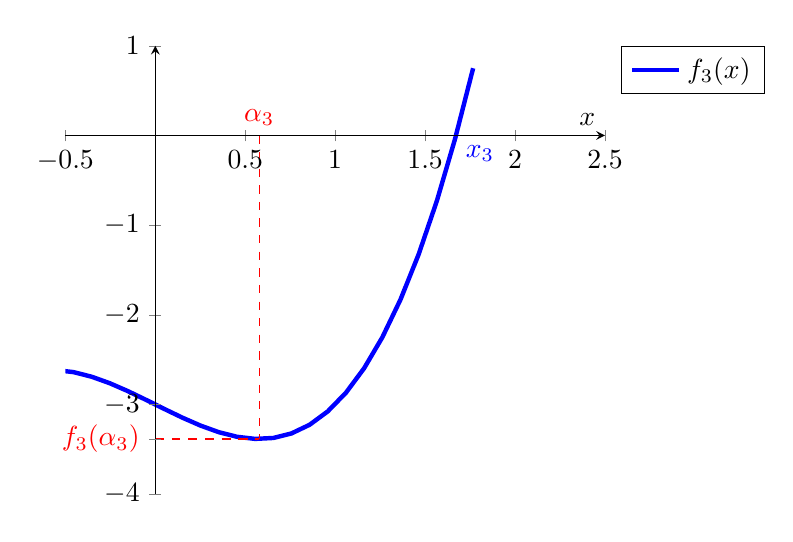
\begin{tikzpicture}
				\begin{axis}
					[
						xlabel=$x$,
						xmin=-0.5, xmax=2.5,
						ymin=-4, ymax=1,
						legend pos=outer north east,
						axis lines=center,
						axis on top=true,
						samples=100,
						extra y ticks={-3.38490017946},
						extra y tick labels={\color{red}$f_{3}(\alpha_{3})$}
					]
					\addplot[blue, ultra thick, restrict y to domain=-4:1] {x^3-x-3};
					\addplot[red, dashed, domain=0:0.57735] {-3.38490017946};
					\addplot[red, dashed, domain=0:0.57735] coordinates {(0.57735,0)(0.57735,-3.38490017946)};
					\node[anchor=north west, color=blue] at (axis cs: 1.6717,0) {$x_{3}$};
					\node[anchor=south, color=red] at (axis cs: 0.57735,0) {$\alpha_{3}$};
					\legend{$f_{3}(x)$}
				\end{axis}
			\end{tikzpicture}
			\caption{$x\mapsto x^{3}-x-3$ a exactement un zéro sur $\R_{+}$.}
		\end{figure}

		\item On a $x_{n}^{n}=x_{n}+n\leqslant2+n$ donc 
		$$1\leqslant x_{n}\leqslant(2+n)^{\frac{1}{n}}=e^{\frac{1}{n}\ln(2+n)}\xrightarrow[n\to+\infty]{}1$$
		Donc 
		$$\boxed{\lim\limits_{n\to+\infty}x_{n}=1}$$

		\item On peut poser $x_{n}=1+\varepsilon_{n}$ avec $\varepsilon_{n}>0$ et $\lim\limits_{n\to+\infty}\varepsilon_{n}=0$. On a 
		$$(1+\varepsilon_{n})^{n}=1+\varepsilon_{n}+n$$
		donc 
		$$n\ln(1+\varepsilon_{n})=\ln(1+\varepsilon_{n}+n)=\ln(n)+\underbrace{\ln\Bigl(1+\frac{1+\varepsilon_{n}}{n}\Bigr)}_{\underset{n\to+\infty}{\sim}\frac{1}{n}}$$
		et donc 
		$$\varepsilon_{n}\underset{n\to+\infty}{\sim}\frac{\ln(n)}{n}$$

		On a donc 
		$$x_{n}=1+\frac{\ln(n)}{n}+o\Bigl(\frac{\ln(n)}{n}\Bigr)$$

		On a enfin 
		$$(1+\varepsilon_{n})^{n}=1+\varepsilon_{n}+n=1+n+\frac{\ln(n)}{n}+o\Bigl(\frac{\ln(n)}{n}\Bigr)$$
		d'où
		\begin{align*}
			\ln(1+\varepsilon_{n})
			&=\frac{1}{n}\ln(n+1+\frac{\ln(n)}{n}+o\Bigl(\frac{\ln(n)}{n}\Bigr))\\
			&=\frac{1}{n}\Bigl[\ln(n)+\ln\Bigl(1+\frac{1}{n}+\underbrace{\frac{\ln(n)}{n^{2}}+o\Bigl(\frac{\ln(n)}{n^{2}}\Bigr)}_{=~o\bigl(\frac{1}{n}\bigr)}\Bigr)\Bigr]\\
			&=\frac{\ln(n)}{n}+\frac{1}{n^{2}}+o\Bigl(\frac{1}{n^{2}}\Bigr)
		\end{align*}
		donc 
		$$1+\varepsilon_{n}=e^{\frac{\ln(n)}{n}+\frac{1}{n^{2}}+o\Bigl(\frac{1}{n^{2}}\Bigr)}=1+\frac{\ln(n)}{n}+\frac{\ln(n)^{2}}{2n^{2}}+o\Bigl(\frac{\ln(n)^{2}}{n^{2}}\Bigr)$$
		puis
		$$\varepsilon_{n}=\frac{\ln(n)}{n}+\frac{\ln(n)^{2}}{2n^{2}}+o\Bigl(\frac{\ln(n)^{2}}{n^{2}}\Bigr)$$
		et ainsi
		$$\boxed{x_{n}=1+\frac{\ln(n)}{n}+\frac{\ln(n)^{2}}{2n^{2}}+o\Bigl(\frac{\ln(n)^{2}}{n^{2}}\Bigr)}$$
	\end{enumerate}
\end{solution}

\begin{solution}
	On note 
	$$v_{n}=\lim\limits_{n\to+\infty}\frac{u_{n}a_{0}+u_{n-1}a_{1}+\dots+u_{0}a_{n}}{u_{0}+\dots+u_{n}}$$

	Si pour tout $n\in\N$, $a_{n}=a$ alors $v_{n}=a\xrightarrow[n\to+\infty]{}a$. De manière générale, on a 
	$$v_{n}-a=v_{n}-a\frac{u_{n}+\dots+u_{0}}{u_{0}+\dots+u_{n}}=\frac{\sum_{k=0}^{n}u_{n-k}(a_{k}-a)}{u_{0}+\dots+u_{n}}$$

	Ainsi,
	$$\vert u_{n}-a\vert\leqslant\frac{\sum_{k=0}^{n}u_{n-k}\vert a_{k}-a\vert}{u_{0}+\dots+u_{n}}$$

	Soit $\varepsilon>0$. Il existe $N\in\N$ tel que pour tout $k\geqslant N$, $\vert a_{k}-a\vert\leqslant\frac{\varepsilon}{2}$. Comme $(a_{k})_{k\in\N}$ converge, on note $M=\sup\limits_{k\in\N}\vert a_{k}-a\vert$. Soit $n\geqslant N$, on a 
	\begin{align*}
		\vert v_{n}-a\vert
		&\leqslant\frac{\sum_{k=0}^{N-1}u_{n-k}\vert a_{k}-a\vert+\sum_{k=N}^{n}\vert a_{k}-a\vert}{u_{0}+\dots+u_{n}}\\
		&\leqslant\frac{\sum_{k=n-N+1}^{n}u_{k}M}{u_{0}+\dots+u_{n}}+\underbrace{\frac{\sum_{k=N}^{n}u_{n-k}\frac{\varepsilon}{2}}{u_{0}+\dots+u_{n}}}_{\leqslant\frac{\varepsilon}{2}}
	\end{align*}
	car les $u_{i}$ sont positifs.

	On remarque enfin que 
	$$
	\begin{array}[]{rcl}
		u_{n} &=& o(u_{0}+\dots+u_{n})\\
		u_{n-1} &=& o(u_{0}+\dots+u_{n-1})=o(u_{0}+\dots+u_{n})\\
		\vdots & &\\
		u_{n-N+1}=o(u_{0}+\dots+u_{n})
	\end{array}
	$$

	Donc 
	$$M\frac{\sum_{k=n-N+1}^{n}u_{k}}{u_{0}+\dots+u_{n}}\xrightarrow[n\to+\infty]{}0$$
	et il existe $N'\in\C$ tel que pour tout $n\geqslant N'$, on a 
	$$M\frac{\sum_{k=n-N+1}^{n}u_{k}}{u_{0}+\dots+u_{n}}\leqslant\frac{\varepsilon}{2}$$
	et donc pour tout $n\geqslant\max(N,N')$, on a $\vert v_{n}-a\vert\leqslant\frac{\varepsilon}{2}$ et ainsi 
	$$\boxed{\lim\limits_{n\to+\infty}v_{n}=a}$$
\end{solution}

\begin{solution}
	\phantom{}
	\begin{enumerate}
		\item Pour $n\geqslant2$, (iii) donne 
		$$x-\frac{a_{2}}{2}-\dots-\frac{a_{n}}{n!}=\sum_{k=n+1}^{+\infty}\frac{a_{k}}{k!}$$
		Ainsi,
		$$0\leqslant x-\frac{a_{2}}{2}-\dots-\frac{a_{n}}{n!}<\sum_{k=n+1}^{+\infty}\frac{k-1}{k!}=\sum_{k=n+1}^{+\infty}\frac{1}{(k-1)!}-\frac{1}{k!}=\frac{1}{n!}$$
		où l'inégalité est stricte d'après (ii). Pour $n\geqslant2$, on a 
		$$x-\frac{a_{2}}{2}<\frac{1}{2!}$$
		donc 
		$$0\leqslant 2x-\underbrace{a_{2}}_{\in\N}<1$$
		Donc $a_{2}=\lfloor 2x\rfloor$.
		On a ensuite 
		$$0\leqslant n!\Bigl(x-\frac{a_{2}}{2}-\dots-\frac{a_{n-1}}{(n-1)!}\Bigr)-\underbrace{a_{n}}_{\in\N}<1$$
		donc 
		$$\boxed{a_{n}=\Biggl\lfloor n!\Bigl(x-\frac{a_{2}}{2}-\dots-\frac{a_{n-1}}{(n-1)!}\Bigr)\Biggr\rfloor}$$

		On a donc bien unicité.

		Soit maintenant $(a_{n})_{n\in\N}$ définie comme ci-dessus. On a, pour tout $n\geqslant2$, on a 
		$$0\leqslant n!\Bigl(x-\frac{a_{2}}{2}-\dots-\frac{a_{n-1}}{(n-1)!}\Bigr)-\underbrace{a_{n}}_{\in\N}<1$$
		Or 
		$$0-\frac{a_{2}}{2}-\dots-\frac{a_{n-1}}{(n-1)!}\leqslant\frac{1}{(n-1)!}$$
		donc 
		$$a_{n}\in\{0,\dots,n-1\}$$
		et (i) est vérifié.

		On a 
		$$0\leqslant x-\sum_{k=2}^{n}\frac{a_{k}}{k!}<\frac{1}{n!}\xrightarrow[n\to+\infty]{}0$$
		donc (iii) est vérifié, et supposons qu'il existe $n_{0}\geqslant2$ tel que pour tout $m\geqslant n_{0}+1$, on a $a_{m}=m-1$.
		Alors 
		$$x=\sum_{k=0}^{n_{0}}\frac{a_{k}}{k!}+\sum_{k=n_{0}+1}^{+\infty}\frac{k-1}{k!}$$
		et
		$$x-\sum_{k=0}^{n_{0}}\frac{a_{k}}{k!} = \sum_{k=n_{0}+1}^{+\infty}\frac{k-1}{k!}=\frac{1}{n_{0}!}$$
		donc 
		$$n_{0}!\Bigl(x-\sum_{k=0}^{n_{0}}\frac{a_{k}}{k!}\Bigr)=1$$
		et 
		$$n_{0}!\Bigl(x-\sum_{k=0}^{n_{0}-1}\frac{a_{n_{0}-1}}{(n_{0}-1)!}\Bigr)-a_{n_{0}}=1$$
		En prenant la partie entière, on a donc $0=1$ ce qui est absurde.

		Donc (ii) est vérifié.
	
		\item S'il existe $n_{0}\in\N$ tel que pour tout $n\geqslant n_{0}$, $a_{n}=0$ alors $x\in\Q$.
		
		Si $x=\frac{p}{q}\in\Q$, on a 
		$$x=\frac{a_{2}}{2}+\dots+\frac{a_{n}}{n!}$$
		si et seulement si 
		$$a_{n}=n!\Bigl(x-\frac{a_{2}}{2}-\dots-\frac{a_{n-1}}{(n-1)!}\Bigr)$$
		si et seulement si 
		$$n!\Bigl(x-\frac{a_{2}}{2}-\dots-\frac{a_{n-1}}{(n-1)!}\Bigr)\in\N$$
		ce qui est vrai dès que $n\geqslant q$. Donc pour tout $n > q$, on a $a_{n}=0$ par unicité.

		\item Soit $l\in[-1,1]$. Soit $x\in[0,1[$ avec 
		$$x=\sum_{k=2}^{+\infty}\frac{a_{k}}{k!}$$
		On a alors 
		$$n!2\pi x=\underbrace{\sum_{k=2}^{n}\frac{2\pi a_{k}n!}{k!}}_{\in 2\pi\Z}+\frac{2\pi a_{n+1}}{n+1}+\underbrace{\sum_{k\geqslant n+2}\frac{2\pi a_{k}n!}{k!}}_{=~\varepsilon_{n}}$$
		On a 
		$$0\leqslant \varepsilon_{n} < \frac{2\pi n!}{(n+1)!}=\frac{2\pi}{n+1}\xrightarrow[n\to+\infty]{}0$$
		Donc 
		$$\sin(n!2\pi x)=\sin\Bigl(\frac{2\pi a_{n+1}}{n+1}+\varepsilon_{n}\Bigr)$$
		et il suffit d'avoir, comme $\varepsilon_{n}\xrightarrow[n\to+\infty]{}0$,
		$$\frac{a_{n}}{n}\xrightarrow[n\to+\infty]{}\frac{\arcsin(l)}{2\pi}\in\Bigl[0,\frac{1}{4}\Bigr]$$
		On pose alors 
		$$\boxed{a_{n}=\Biggl\lfloor\frac{n\arcsin(l)}{2\pi}\Biggr\rfloor}$$
		pour $n\geqslant2$ et on a $0\leqslant a_{n}\leqslant \frac{n}{4}<n-1$ pour tout $n\geqslant2$. On a donc le résultat.
	\end{enumerate}
\end{solution}

\begin{remark}
	Il n'y a pas unicité. Par exemple, pour $l=0$, $x=0$ ou $x=\frac{1}{2}$ convient. Plus généralement, pour tout $\frac{p}{q}\in\Q$, pour tout $n\geqslant q$, on a
	$$\sin\Biggl(n!2\pi\Bigl(x+\frac{p}{q}\Bigr)\Biggr)=\sin(n!2\pi x)$$
\end{remark}

\begin{solution}
	Par récurrence, on a $u_{n}>0$ pour tout $n\in\N$.
	Soit \function{g}{\R_{+}}{\R}{x}{2\ln(1+x)-x}
	et \function{f}{\R_{+}}{\R}{x}{2\ln(1+x)}
	$g$ est dérivable est 
	$$g'(x)=\frac{1-x}{1+x}$$
	donc $g$ est croissante sur $[0,1]$ et décroissante sur $[1,+\infty[$. Comme $g(0)=0$ et $\lim\limits_{x\to+\infty}g(x)=-\infty$, d'après le théorème des valeurs intermédiaires, il existe un unique réel $l\in]0,+\infty[$ tel que $g(l)=0$ d'où $f(l)=l$.

	\begin{figure}
		\centering
		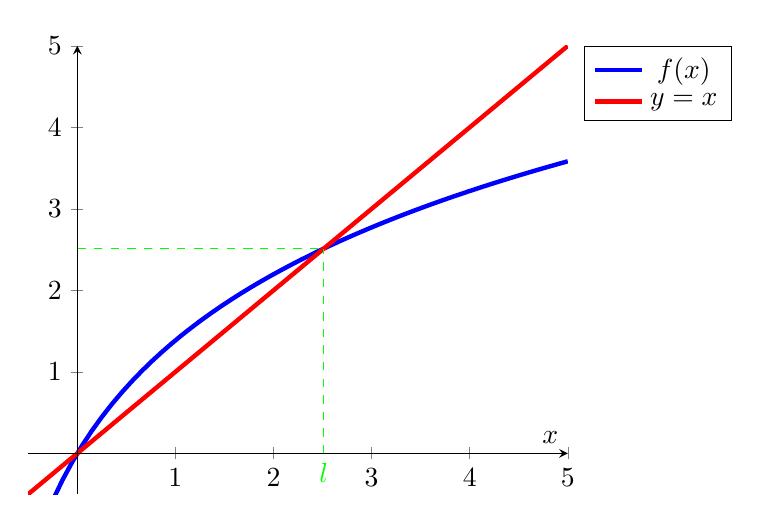
\begin{tikzpicture}
			\begin{axis}[
				xmin=-0.5, xmax=5,
				ymin=-0.5, ymax=5,
				axis lines=center,
				axis on top=true,
				xlabel=$x$,
				samples=100,
				legend pos=outer north east
			]
			\addplot[blue, ultra thick] {2*ln(1+x)};
			\addplot[color=red, ultra thick] {x};
			\addplot[green, dashed, domain=0:2.5128] {2.5128};
			\addplot[green, dashed, domain=0:2.5128] coordinates {(2.5128,0)(2.5128,2.5128)};
			\node[anchor=north, color=green] at (axis cs: 2.5128,0) {$l$};
			\legend{$f(x)$,$y=x$}
			\end{axis}
		\end{tikzpicture}
		\caption{$x\mapsto 2\ln(1+x)$ admet un unique point fixe sur $\R_{+}^{*}$.}
	\end{figure}

	Pour tout $x\in]0,l]$, on a $x\leqslant f(x)\leqslant l$ et pour tout $x>l$, on a $l\leqslant f(x)\leqslant x$.

	Soit $n\geqslant1$. Si $u_{n}\geqslant l$ et $u_{n-1}\geqslant l$, on a $m_{n}=l$ et $M_{n}\in\{u_{n},u_{n-1}\}$. Il vient donc 
	$$u_{n+1}=\frac{1}{2}(f(u_{n})+f(u_{n-1}))\geqslant f(l)=l$$
	et 
	$$u_{n+1}\leqslant\frac{1}{2}(u_{n}+u_{n-1})\leqslant M_{n}$$
	Donc $m_{n+1}=l=m_{n}$ et $M_{n+1}\leqslant M_{n}$.

	Par récurrence, on a pour tout $k\geqslant n$, $u_{k}\geqslant l$ et $(M_{k})_{k\geqslant n}$ converge vers $\lambda\geqslant l$ (car décroissante et plus grande que $l$) et $m_{k}=l$ pour tout $k\geqslant n$.

	De plus pour tout $k\geqslant n$, on a 
	$$u_{k+1}=\frac{1}{2}(f(u_{k})+f(u_{k-1}))\leqslant f(M_{k})$$
	car $f$ est croissante et donc 
	$$u_{k+2}\leqslant f(M_{k+1})\leqslant f(M_{k})$$
	Par passage à la limite, on a $\lambda\leqslant f(\lambda)$ donc $\lambda=f(\lambda)$ et donc $\lambda=l$. Or pout tout $k\geqslant n$, on a 
	$$\underbrace{m_{k}}_{=~l}\leqslant u_{k}\leqslant M_{k}\xrightarrow[k\to+\infty]{}l$$
	donc 
	$$\boxed{u_{k}\xrightarrow[k\to+\infty]{}l}$$

	S'il existe $n_{0}\in\N^{*}$ tel que $u_{n_{0}-1}\geqslant l$ et $u_{n_{0}}\geqslant l$ alors $\lim\limits_{n\to+\infty}u_{n}=l$. Or même s'il existe $n_{1}\in\N^{*}$ tel que $u_{n_{1}-1}\leqslant l$ et $u_{n_{1}}\leqslant l$, alors on inverse les rôles de $M_{n_{1}}$ et $m_{n_{1}}$.

	Si pour tout $n\in\N$,
	$$(u_{n}-l)(u_{n+1}-l)\leqslant 0$$
	Supposons par exemple $u_{0}\geqslant l$ et $u_{1}\leqslant l$. Alors 
	$$0\leqslant u_{2}-l\leqslant\frac{u_{0}-l}{2}$$
	et par récurrence, pour tout $k\in\N$, on a $0\leqslant u_{2k}-l\leqslant\frac{u_{0}-l}{2^{k}}$.
	Donc $u_{2k}\xrightarrow[k\to+\infty]{}l$ et de même $u_{2k+1}\xrightarrow[k\to+\infty]{}l$ (par valeurs inférieures). Donc 
	$$\boxed{u_{k}\xrightarrow[k\to+\infty]{}l}$$
\end{solution}

\begin{solution}
	Soit $(\theta,\theta')\in[2,2\pi[^{2}$ tel que 
	$$\lim\limits_{k\to+\infty}e^{\i px_{n}}=e^{\i \theta}$$ et 
	$$\lim\limits_{k\to+\infty}e^{\i qx_{n}}=e^{\i \theta'}$$
	Soient $x,x'$ deux valeurs d'adhérence de $(x_{n})_{n\in\N}$ distinctes. On a 
	$$
	\left\{
		\begin{array}[]{l}
			e^{\i px}=e^{\i \theta}=e^{\i px'}\\
			e^{\i qx}=e^{\i \theta'}=e^{\i qx'}
		\end{array}
	\right.
	$$

	Il existe $(k,k')\in\Z^{2}$ tel que 
	$$
	\left\{
		\begin{array}[]{l}
			px=px'+2k\pi\\
			qx=qx'+2k\pi
		\end{array}
	\right.
	$$
	et donc $p(x-x')=2k\pi$ et $q(x-x')=2k'\pi$ et alors $\frac{p}{q}\in\Q$ ce qui contredit l'hypothèse. Donc $(u_{n})_{n\in\N}$ possède une unique valeur d'adhérence. Comme elle est bornée,
	$$\boxed{(x_{n})_{n\in\N}\text{ converge.}}$$

	Si $(x_{n})_{n\in\N}$ n'est pas bornée, on peut prendre 
	$$\boxed{x_{n}=n!}$$
	On a 
	$$e^{2\i \pi n!}=1$$
	et 
	$$n!e=n!\sum_{k=0}^{+\infty}\frac{1}{k!}=\underbrace{\sum_{k=0}^{n}\frac{n!}{k!}}_{\in\N}+\underbrace{\sum_{k=n+1}^{+\infty}\frac{n!}{k!}}_{\xrightarrow[k\to+\infty]{}0}$$
	
	Si on veut $x_{n}$ divergente dans $\overline{\R}$, on peut prendre 
	$$\boxed{x_{n}=(-1)^{n}n!}$$
\end{solution}

\begin{solution}
	\phantom{}
	\begin{enumerate}
		\item On a $$\binom{n}{k}=\frac{n!}{k!(n-k)!}=\frac{n(n-1)\dots(n-k+1)}{k!}\leqslant\boxed{\frac{n^{k}}{k!}}$$
		\item On a 
		$$\left(1+\frac{z}{n}\right)^{n}=\sum_{k=0}^{n}\binom{n}{k}\left(\frac{z}{n}\right)^{k}$$
		donc 
		\begin{align*}
			\left|\sum_{k=0}^{n}\frac{z^{k}}{k!}-\binom{n}{k}\frac{z^{k}}{n^{k}}\right|
			&\leqslant\sum_{k=0}^{n}\vert z\vert^{k}\underbrace{\left|\frac{1}{k!}-\binom{n}{k}\frac{1}{n^{k}}\right|}_{\geqslant0}\\
			&\leqslant\sum_{k=0}^{n}\frac{\left|z\right|^{k}}{k!}-\sum_{k=0}^{n}\binom{k}{n}\frac{\left|z\right|^{k}}{n^{k}}\\
			&\boxed{=\sum_{k=0}^{n}\frac{\left|z\right|^{k}}{k!}-\left(1+\frac{\left|z\right|}{n}\right)^{n}}
		\end{align*}

		\item On sait que 
		$$\sum_{k=0}^{n}\frac{\left|z\right|^{k}}{k!}\xrightarrow[k\to+\infty]{}e^{\left|z\right|}$$
		et 
		$$\left(1+\frac{\left|z\right|}{n}\right)^{n}=e^{n\ln\left(1+\frac{\left|z\right|}{n}\right)}=e^{n\left(\frac{\left|z\right|}{n}+o\left(\frac{\left|z\right|}{n}\right)\right)}=e^{\left|z\right|}e^{o\left(1\right)}\xrightarrow[n\to+\infty]{}e^{\left|z\right|}$$
		
		En reportant dans la question précédente, on a donc 
		$$\boxed{\lim\limits_{n\to+\infty}\left(1+\frac{z}{n}\right)^{n}=\sum_{k=0}^{+\infty}\frac{z^{k}}{k!}=e^{z}}$$
	\end{enumerate}
\end{solution}

\begin{remark}
	Une autre méthode est d'écrire, pour $z=a+\i b$, 
	$$1+\frac{z+\i b}{n}=1+\frac{a}{n}+\i\frac{b}{n}=\rho_{n}e^{\i\theta_{n}}$$.
	On a alors 
	$$\left|1+\frac{a+\i b}{n}\right|=\sqrt{\left(1+\frac{a}{n}\right)^{2}+\frac{b^{2}}{n^{2}}}=\rho_{n}$$
	et alors 
	\begin{align*}
		\rho_{n}^{n}
		&=\left|\left(1+\frac{z}{n}\right)\right|^{n}\\
		&=e^{\frac{n}{2}\ln\left(\left(1+\frac{a}{n}\right)^{2}+\frac{b^{2}}{n^{2}}\right)}\\
		&=e^{\frac{n}{2}\ln\left(1+\frac{2a}{n}+o\left(\frac{1}{n}\right)\right)}\\
		&=e^{a+o\left(1\right)}\xrightarrow[n\to+\infty]{}e^{a}=\left|e^{z}\right|
	\end{align*}

	On écrit ensuite 
	$$1+\frac{a+\i b}{n}=\rho_{n}\Bigl(\underbrace{\frac{1+\frac{a}{n}}{\rho_{n}}}_{=~\cos(\theta_{n})}+\i\underbrace{\frac{b}{n\rho_{n}}}_{=~\sin(\theta_{n})}\Bigr)$$
	On a alors
	$$\lim\limits_{n\to+\infty}\frac{b}{n\rho_{n}}=0\text{ et }\lim\limits_{n\to+\infty}\frac{1+\frac{a}{n}}{\rho_{n}}=1$$
	On peut imposer $\theta_{n}\in]-\pi,\pi]$ et il existe alors $N\in\N$ tel que pour tout $n\geqslant N$, $\cos(\theta_{n})\geqslant0$. Pour $n\geqslant N$, on a alors $\theta_{n}\in\left[-\frac{\pi}{2},\frac{\pi}{2}\right]$ donc 
	$$\theta_{n}=\arcsin\left(\frac{b}{n\rho_{n}}\right)$$
	et $n\theta_{n}=n\arcsin\left(\frac{b}{n\rho_{n}}\right)\underset{n\to+\infty}{\sim}b$. Finalement, on a bien 
	$$\left(1+\frac{z}{n}\right)^{n}=\rho_{n}^{n}e^{\i\theta_{n}}\xrightarrow[n\to+\infty]{}e^{a}e^{\i b}=e^{z}$$
\end{remark}

\begin{solution}
	Pour tout $n\geqslant2$, $u_{n}>0$. On a 
	$$u_{n+1}=\underbrace{\frac{\sqrt{n+1}-1}{\sqrt{n+1}+1}}_{<1}u_{n}$$
	donc $(u_{n})_{n\in\N}$ est décroissante donc converge. On a 
	$$\ln(u_{n})=\sum_{k=2}^{n}\underbrace{\ln\Bigl(1-\frac{1}{\sqrt{k}}\Bigr)-\ln\Bigl(1+\frac{1}{\sqrt{k}}\Bigr)}_{=~v_{k}}<0$$
	Ensuite, 
	$$v_{k}=-\frac{1}{\sqrt{k}}-\frac{1}{\sqrt{k}}+o\left(\frac{1}{\sqrt{k}}\right)\underset{k\to+\infty}{\sim}-\frac{2}{\sqrt{k}}$$

	Comme $\sum_{k\geqslant2}\frac{1}{\sqrt{k}}$ diverge, on a $\lim\limits_{n\to+\infty}\ln(u_{n})=-\infty$.

	Ainsi, 
	$$\boxed{\lim\limits_{n\to+\infty}u_{n}=0}$$

	On a ensuite 
	$$u_{n}=\exp\left(\sum_{k=2}^{n}\left[\ln\left(1-\frac{1}{\sqrt{k}}\right)-\ln\left(1+\frac{1}{\sqrt{k}}\right)\right]\right)$$
	et 
	$$\ln\left(1\pm\frac{1}{\sqrt{k}}\right)=\pm\frac{1}{\sqrt{k}}-\frac{1}{2k}+O\left(\frac{1}{k^{\frac{3}{2}}}\right)$$
	Donc 
	$$v_{k}=-\frac{2}{\sqrt{k}}+O\left(\frac{1}{k^{\frac{3}{2}}}\right)$$
	Le terme dans le $O$ est le terme générale d'une série absolument convergent donc convergent, on note ce terme $\alpha_{k}$. On a alors 
	$$\sum_{k=2}^{n}v_{k}=\sum_{k=2}^{n}\left(-\frac{2}{\sqrt{k}}+\alpha_{k}\right)=-2\sum_{k=2}^{n}\frac{1}{\sqrt{k}}+\underbrace{\sum_{k=2}^{+\infty}\alpha_{k}}_{=~C}+o\left(1\right)$$
	Par comparaison série-intégrale, on a 
	$$\sum_{k=2}^{n}\frac{1}{\sqrt{k}}\underset{k\to+\infty}{\sim}\int_{2}^{n}\frac{dt}{\sqrt{t}}\underset{k\to+\infty}{\sim}2\sqrt{n}$$

	Posons 
	$$w_{n}=\sum_{k=2}^{n}\frac{1}{\sqrt{k}}-2\sqrt{n}$$
	On étudie la série de terme général $w_{n}-w_{n-1}$. On a 
	\begin{align*}
		w_{n}-w_{n-1}
		&=\frac{1}{\sqrt{n}}-2\left(\sqrt{n}-\sqrt{n-1}\right)\\
		&=\frac{1}{\sqrt{n}}-2\left(1-\sqrt{1-\frac{1}{n}}\right)\\
		&=\frac{1}{\sqrt{n}}-2\left(1-\left(1-\frac{1}{2n}+O\left(\frac{1}{n^{2}}\right)\right)\right)\\
		&=\frac{1}{\sqrt{n}}-\frac{\sqrt{n}}{n}+O\left(\frac{1}{n^{\frac{3}{2}}}\right)\\
		&=O\left(\frac{1}{n^{\frac{3}{2}}}\right)
	\end{align*}

	Donc la série de terme général $w_{n}-w_{n-1}$ converge et ainsi $(w_{n})_{n\geqslant2}$ converge: il existe $C'\in\R$ tel que 
	$$\sum_{k=2}^{n}\frac{1}{\sqrt{n}}=2\sqrt{n}+C'+o\left(1\right)$$

	On a donc 
	$$\ln(u_{n})=\sum_{k=2}^{n}v_{k}=-4\sqrt{n}-2C'+C+o\left(1\right)$$
	Ainsi, 
	$$u_{n}=\exp\left(-4\sqrt{n}-2C'+C+o\left(1\right)\right)\underset{n\to+\infty}{\sim}Ke^{-4\sqrt{n}}$$
	où $K=e^{-2C'+C}>0$.

	Donc 
	$$u_{n}^{\alpha}\underset{n\to+\infty}{\sim}K^{\alpha}e^{-4\alpha\sqrt{n}}$$

	Si $\alpha\leqslant0$, $\lim\limits_{n\to+\infty}u_{n}^{\alpha}\not\to 0$
	donc 
	$$\boxed{\sum u_{n}^{\alpha}\text{ diverge.}}$$

	Si $\alpha>0$, $u_{n}^{\alpha}=o\left(\frac{1}{n^{2}}\right)$ donc d'après le critère de Riemann, 
	$$\boxed{\sum u_{n}^{\alpha}\text{ converge.}}$$
\end{solution}

\begin{solution}
	Soit $S_{n}=\sum_{k=0}^{n}u_{k}$. On a 
	$$u_{n+1}+\dots+u_{2n}\geqslant nu_{2n}\geqslant0$$

	Si $(S_{n})$ converge alors $S_{2n}-S_{n}\xrightarrow[n\to+\infty]{}0$. Alors $\lim\limits_{n\to+\infty}nu_{2n}=0$ et $\lim\limits_{n\to+\infty}2n u_{2n}=0$.

	Comme on a $(2n+1)u_{2n}\geqslant (2n+1)u_{2n+1}\geqslant0$, on a aussi $\lim\limits_{n\to+\infty}(2n+1) u_{2n}=0$. Finalement, on a bien 
	$$\boxed{\lim\limits_{n\to+\infty}nu_{n}=0\text{ et donc }u_{n}=o\left(\frac{1}{n}\right)}$$

	Si $\left\{p\in\N \middle|pu_{p}\geqslant1 \right\}$ est infini, alors $u_{p}\neq o\left(\frac{1}{p}\right)$ donc 
	$$\boxed{\sum u_{p}\text{ diverge.}}$$
\end{solution}

\begin{remark}
	Ce n'est pas vrai si $(u_{n})_{n\in\N}$ n'est pas décroissante, par exemple si $u_{n}=\frac{1}{n}$ si $n$ est un carré et 0 sinon.
\end{remark}